\documentclass[notitlepage]{article}
\usepackage{graphicx}
\usepackage{authblk}
\usepackage{url}
\usepackage[inline,shortlabels]{enumitem}
\usepackage[square,numbers]{natbib}
% \usepackage{natbib}
\usepackage[nomarkers,nolists]{endfloat}
\renewcommand{\efloatseparator}{\mbox{}} % multiple figures per page
\usepackage[letterpaper,left=1in,right=1in,top=1in,bottom=1in,footskip=0.25in]{geometry}
\usepackage{csvsimple}
\usepackage{multirow}
\usepackage[table]{xcolor}
\linespread{1.5}
\bibliographystyle{unsrtnat}

\begin{document}

\title{Removing nonlinear batch effects from gene-expression data using adversarial deep neural networks}
\author[1]{Jonathan B. Dayton}
\author[1]{Stephen R. Piccolo}
\affil[1]{Department of Biology, Brigham Young University, Provo, UT 84602 USA}
\date{}

\maketitle

\begin{abstract}
	Many biological studies, particularly studies involving the genetics of human disease, could discover items of greater statistical and biological significance if performed with larger data sets.
	Many data sets are publicly available and could be combined in order to increase these studies' significance, but even when the same type of data are collected by multiple studies, minor differences in collection methodologies and environments can lead to confounding effects in the data which can in turn cause incorrect results.
	In order to combine date produced under different conditions, we applied deep learning to remove these effects and combine gene expression datasets.
	We created an adversarial variational autoencoder in order to remove confounding effects from the data while minimizing the amount of change to the input data.
	We tested the model on artificially constructed data and commonly used real gene expression datasets and compared the output with the output from other common batch adjustment algorithms.
	We also applied the model to remove the cancer-type-specific signal from pan-cancer expression data.
	Our software is available at \url{https://github.com/jdayton3/Confounded} to enable other scientists to remove confounding effects from their own data using our methodologies.
\end{abstract}

\section{Background} \label{sec:background}

When working with gene expression data, problems can arise from combining data from multiple sources.
For example, if two labs sequence and quantify the same RNA samples for the same lung cancer patients but use different equipment to do so, each lab will come up with slightly different measurements (see Figure \ref{fig:workflow}).
% Is this ^ the best way to reference figures?
If a third party were to then study the patients using data from both labs, the differences in measurements could alter their analysis.
These systemic effects are known as ``batch effects'' and are understood to have a nontrivial impact on high-throughput expression data \citep{leek_tackling_2010}.
In one study, researchers found that, contrary to previous knowledge, expression values from mice and humans clustered more closely by species than by tissue type \citep{yue_comparative_2014};
however, referees showed in a rebuttal that when accounting for batch effects, these data actually clustered more closely by tissue type, as initially expected \citep{gilad_reanalysis_2015}.
Systemic bias can be even more pronounced when using data collected from different tissue types and can skew results, such as in pan-cancer analyses \citep{dayton_classifying_2017-1}.

\begin{figure}
	\centering
	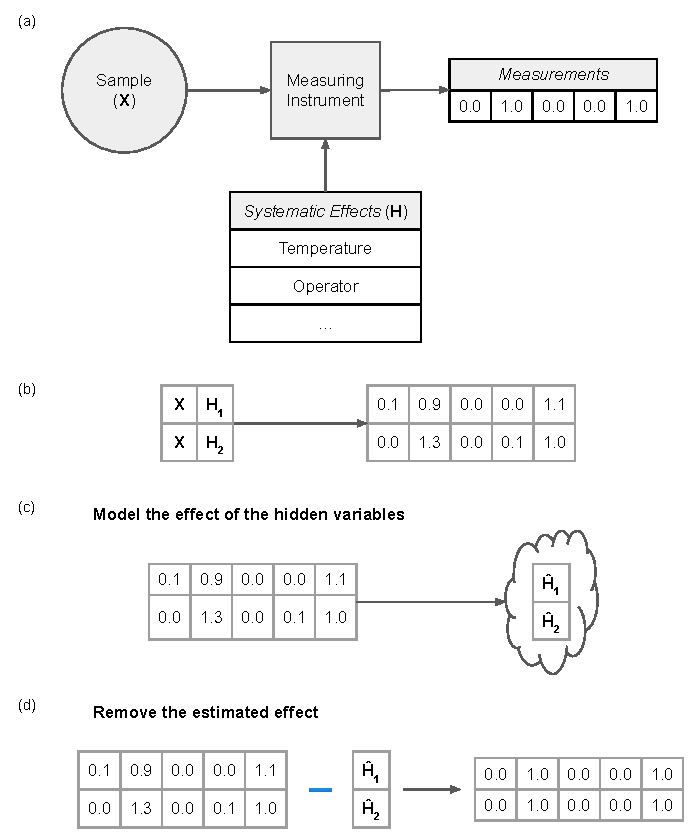
\includegraphics[width=\columnwidth]{figures/final/adjuster_workflow.pdf}
	\caption[]{\textbf{Batch adjustment justification and steps}
	\begin{enumerate*}[(a)]
		\item When measurements are collected from a sample ($X$), systemic effects ($H$) also affect the measurements.
		\item If data from the same sample $X$ is measured under two different conditions, $H_1$ and $H_2$, we may obtain slightly different measurements.
		\item In order to normalize batches of data relative to one another, we first estimate the effect of the hidden variables based on differences in measurements between batches.
		\item Second, we remove the estimated effects in order to normalize the batches relative to one another.
	\end{enumerate*}
	}
	\label{fig:workflow}
\end{figure}

Several methods exist for removing batch effects from gene expression datasets.
Two commonly used methods are ComBat \citep{johnson_adjusting_2007} and SVA \citep{leek_capturing_2007}.
ComBat uses an empirical Bayes method to estimate batch effect parameters and then uses linear regression to remove the effects, and SVA uses singular value decomposition to model batch effects which can then be accounted for in statistical analyses.
Since both of these methods use linear adjustments to remove batch effects, they cannot account for nonlinear effects, such as complex interactions in gene pathways in response to environmental changes.
As machine learning becomes more common in biological research, these nonlinear batch effects become more troublesome since many machine learning algorithms can successfully identify complex interactions between variables.
Advances in neural networks have introduced new ways to account for higher-order, nonlinear relationships in data.
These networks have proven effective in removing irrelevant, domain-specific signal in credit rating, online reviews, and image recognition tasks \citep{louizos_variational_2015}.
Recent work \cite{shaham_removal_2017,shaham_batch_2018,upadhyay_removal_2019} has applied neural networks to batch effects.
However, these recent programs have several items that complicate their usability on many real-world datasets:
they require that the input data only contains two batches, that the batches are sufficiently large, and that the batches are perfectly balanced.
These requirements rarely hold in existing datasets; for example, the bladderbatch dataset used in the documentation for the R sva package \cite{leek_bladderbatch_2017,leek_sva_2017} has 5 batches, only 57 samples, and between 4 and 19 samples per batch.
Additionally, the metrics these studies have used to validate results don't test whether complex interactions still remain in the data.

To address these issues, we implemented a deep neural network approach to batch correction that works on real-world datasets, and we calculated batch removal measurements based on machine learning algorithms to test for remaining nonlinear effects.
Artificial neural networks are a machine learning tool inspired by the way human brains function; input values pass through layers of linear and nonlinear functions, the final output values are measured against objectives, and the layers of functions are adjusted to bring the outputs closer to the objectives.
This process is repeated until the outputs are sufficiently close to their targets \citep{schmidhuber_deep_2015}.
Research has shown that neural networks are effective in working with gene expression data; for example, neural networks have been applied to extract biologically relevant latent spaces in RNA-Seq data with as few as 10,000 samples \citep{way_extracting_2017}, and some researchers have used that latent space to generate realistic synthetic biomedical data for other scientific studies \citep{beaulieu-jones_privacy-preserving_2017}.
Autoencoders are a type of neural network that encode and then reconstruct their input, and their traditional objective function is to construct the output to be as similar to the input as possible \citep{hinton_reducing_2006}.
Neural networks have historically decreased in effectiveness when working with data from multiple research domains \citep{ganin_domain-adversarial_2015}, in part because they may learn based on dataset-specific confounding effects (e.g. which researcher collected the data) instead of learning based on practically meaningful causal effects (e.g. which gene is consistently upregulated in a disease) \citep{louizos_causal_2017-2}.
Recently, researchers have experimented with discouraging neural networks from learning based on domain-specific information by giving them two objective functions:
1. to learn as much as possible about the input data and
2. to forget any patterns that help distinguish between domains \citep{ganin_domain-adversarial_2015,tzeng_deep_2014-2}.
This type of dual objective function has been used in conjunction with autoencoders \citep{louizos_variational_2015} where the autoencoder is ``rewarded'' for reconstructing the input faithfully, but ``penalized'' for retaining class-specific patterns in the output.

In this study, we present Confounded, an adversarial autoencoder that identifies and removes effects between different batches.
We test the hypothesis that using an adversarial neural network can correct for batch effects more completely than previous tools do.
We also explore the extent to which batch effects still remain in different datasets after adjustment with various algorithms, and we present a framework to assess the extent to which batch effects remain after adjustment using various classification algorithms.

\section{Methods} \label{sec:methods}

\subsection{Network Structure}

We used an adversarial autoencoder network to model and remove the batch effects.
We structured this network in two parts: a variational autoencoder \cite{louizos_variational_2015} to replicate the input (expression) data and a discriminator to detect remaining batch effects in the autoencoder's output.
By penalizing the autoencoder for the discriminator's success, the autoencoder subnetwork learned over the course of training to output the expression data free of batch effects.
We implemented the neural network in TensorFlow 1.11.0 \cite{abadi_tensorflow_2015} with Python 3.6 \cite{python_software_foundation_python_2019}.
All layers in the network were fully connected and all activation functions were ReLUs \cite{agarap_deep_2018} except the final layers in the autoencoder and the discriminator, which used the sigmoid function.

\begin{figure}
	\centering
	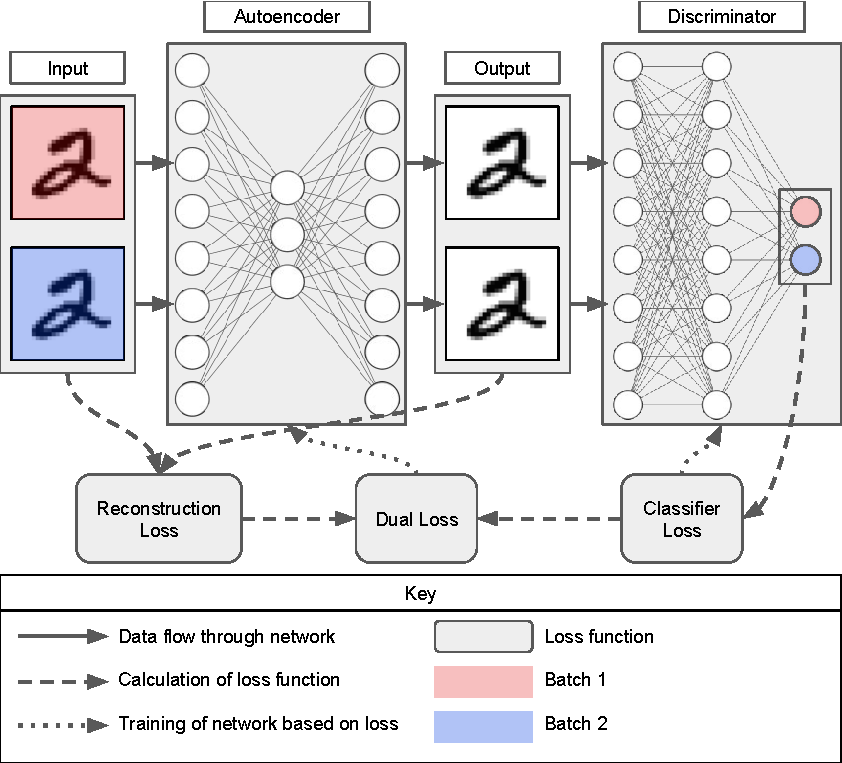
\includegraphics[width=\columnwidth]{figures/final/network.pdf}
	\caption{\textbf{Network architecture} of Confounded.
	Data with batch effects (represented by different colors) are input into an autoencoder.
	The output of the autoencoder is classified by a discriminator network based on batch.
	The autoencoder is then penalized based on the success of the discriminator.
	Over time, the autoencoder learns to output a faithful representation of the data without signal due to batch.}
	\label{fig:network}
\end{figure}

\subsubsection{Autoencoder}

We implemented the variational autoencoder \cite{louizos_variational_2015} described by \citet[Chapter 15]{geron_hands-machine_2017}.
Additional information can be found in our supplementary material.

\subsubsection{Discriminator}

We trained the discriminator to determine the original batch of the autoencoder's output.
The discriminator subnetwork consists of an input layer; four fully connected hidden layers of sizes 1024, 512, 512, and 128, respectively; and an output layer sized based on the number of batches.
In order to combat overfitting and improve training, we also added 50\%-probability dropout \cite{srivastava_dropout_2014} and batch normalization \cite{ioffe_batch_2015} to each layer of the discriminator.
These additions seemed to reduce overfitting in the discriminator.

\subsubsection{Loss functions}

We trained the network using three loss functions.
First, we calculated the autoencoder's loss ($L_A$) by summing the reconstruction loss (sigmoid cross entropy between the autoencoder's input and output) and the latent loss (Kullback-Leibler divergence \cite{kullback_information_1951} of the code layer).
Second, we calculated the discriminator's loss ($L_D$) as sigmoid cross entropy between its output and a one-hot encoding of the samples' batch labels.
Finally, we also trained the autoencoder layers on a combination of the two previous losses,

\begin{equation}
	\label{dual_loss}
	L_{dual} = L_A - \lambda{}(L_D)
\end{equation}

The $\lambda$ value represents a tradeoff parameter for tuning the network's tendency for more faithfully replicating the input or for more completely removing batch effects.
A higher $\lambda$ value indicates that the network should remove batch effects more aggressively, whereas a lower value indicates that the network should instead favor faithfully reconstructing the input data.
We did not optimize $L_A$ directly; instead we trained the autoencoder by optimizing $L_{dual}$.

\subsubsection{Training}

In all cases, we trained the network using the Adam Optimizer \cite{kingma_adam_2014} with a training rate of 0.0001 for 10,000 iterations on mini-batches of size 100.
In each iteration, we optimized on both $L_D$ and $L_{dual}$.
When optimizing $L_D$ (i.e. training the discriminator), we froze the autoencoder's weights, and vice versa.
We trained the network on a 2017 Dell XPS 15 9560 with an 8-core Intel i7-7700HQ CPU and 16 GB of RAM.
For each dataset, training typically took roughly 30 minutes to complete, including the time taken to load the input into memory and to save the output to disk.

\begin{figure}
	\centering
	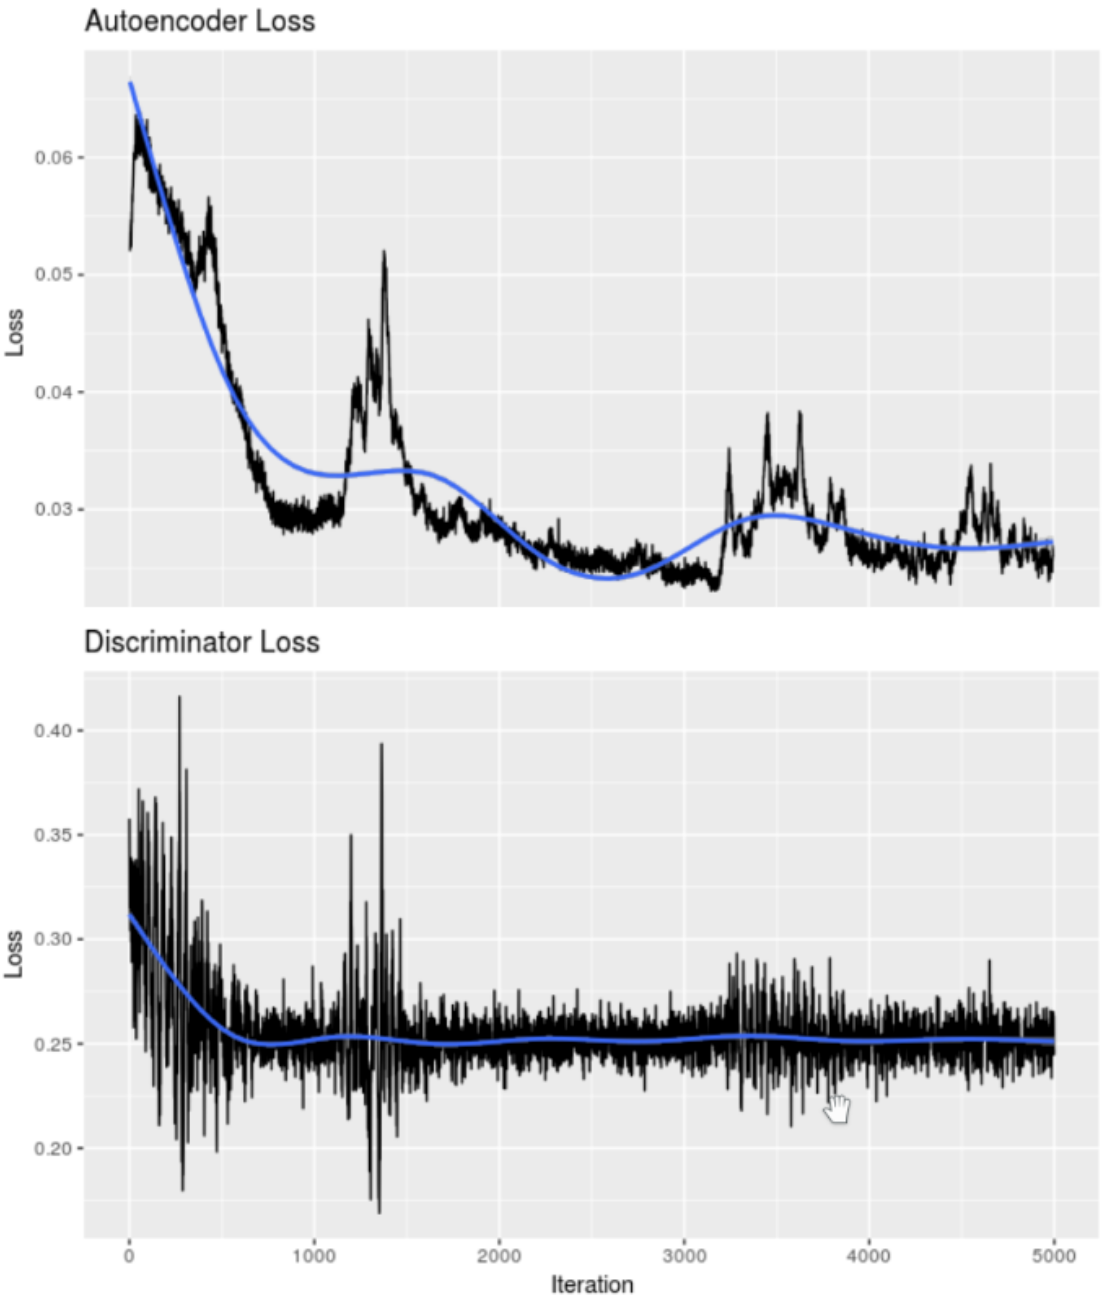
\includegraphics[width=\columnwidth]{figures/rough/training_loss.png}
	\caption{Autoencoder and discriminator loss over time for one run of Confounded.
	Over the course of training, the autoencoder more faithfully replicates the input data.
	The autoencoder also seems to introduce noise (see around iteration 3100) in response to the discriminator's slight improvements.}
	\label{fig:training_loss}
\end{figure}

\subsection{Datasets}

In order to test both theoretical and practical differences between Confounded and previous methods, we compared them for a variety of datasets of varying sizes and type of data measured.

\begin{table}
	\centering
	\begin{tabular}{|p{0.18\linewidth}|p{0.14\linewidth}|p{0.1\linewidth}|p{0.15\linewidth}|p{0.23\linewidth}|p{0.16\linewidth}|}
  \hline
  Dataset         & Dimensions   & Number of Batches & Batch Label      & True Class Label       & Data Type        \\
  \hline
  Bladder Batch   & $57\times22,283$  & 5                 & Batch            & Cancer status          & Microarray       \\
  \hline
  GSE37199        & $93\times20,024$  & 2                 & Plate            & Cancer stage           & Microarray       \\
  \hline
  MNIST           & $10,000\times784$ & 2                 & Artificial batch & Digit                  & Grayscale images \\
  \hline
  TCGA Pan-Cancer & $9,366\times325$  & 25                & Cancer Type      & TP53 mutation presence & RNA-Seq \\
  \hline
\end{tabular}

	\caption{\textbf{Dataset information} for each dataset used.}
	\label{tab:datasets}
\end{table}

\subsubsection{MNIST}

The MNIST digits dataset \cite{lecun_mnist_nodate} is a database of images of handwritten digits that are size-normalized and centered.
It contains 60,000 training images and 10,000 test images.
We used MNIST so we could visually assess how well the true signal (in this case, the shape and digit of each handwritten digit image) was preserved after batch adjustment.
In order to use this dataset, we flattened each 28 by 28 image into a 1D vector of size 784 and put each in a CSV file along with the accompanying digit information.
We limited our dataset to only the 10,000 test images.
Although convolutional layers are typically used when working with image data, we only used fully connected layers even for this image dataset.
In this way, we show that the autoencoder is still able to find and represent spatial relationships without explicitly defining spatial relationships in the model while testing the same network we use on expression data, where no spatial relationships are inherent.

\paragraph{Synthetic Batch Effects}

Because there is no batch information in the MNIST digits dataset, we had to simulate nonlinear batch effects.
To do so, we wrote a Python script to take the MNIST data in, apply a nonlinear effect, and output the adjusted data.
We applied nonlinear effects by iteratively realizing vectors of normally distributed values, multiplying and adding these vectors to the ``expression'' vectors, and applying nonlinearity to the adjusted vector.
We split the image data into two batches while keeping the batches balanced (5,000 images for each batch) and including the same number of each digit in each batch.
We applied the same random vectors to each image in a batch.
Finally, we added random noise to each image in order to prevent images in a batch from being overly similar to each other.

\subsubsection{Bladderbatch}

The bladderbatch dataset is a microarray transcriptomic expression dataset from a study of patients with bladder cancer \cite{dyrskjot_gene_2004}.
It has been made available as an R package \cite{leek_bladderbatch_2017} and is used in the documentation of the sva R package \cite{leek_sva_2017} to illustrate how to batch-adjust using ComBat.
It contains expression values for 57 tissue samples with and without bladder cancer across 5 unbalanced batches.
The dataset has a cancer status (cancerous vs. normal tissue) column, which we used for ``true class'' classification, and a batch column.
Because bladderbatch is such a small dataset in terms of typical deep learning datasets, we selected it as a way to test whether our network was overfitting.

\subsubsection{GSE37199}

The GSE37199 dataset contains Affymetrix microarray gene-expression data from patients with advanced castration-resistant prostate cancer \cite{olmos_prognostic_2012}.
We accessed a version of this data from \url{http://doi.org/10.17605/OSF.IO/SSK3T} that was tidied as part of a curated compendium of human transcriptional biomarker data \cite{golightly_curated_2018}.
It contains expression values for 93 tissue samples categorized as either ``Advanced castration resistant'' or ``good prognosis.''
We used this cancer status variable as the ``true class'' for classification.
It has two types of batch variables: ``plate'' and ``centre.''
We adjusted against the ``plate'' variable because it was more balanced than ``centre'' (with counts of $\{43, 50\}$ compared to $\{27, 66\}$).
The GSE37199 dataset represents a slightly larger dataset than bladderbatch, with only two batches that are closer to being balanced (with batch counts of $\{4, 5, 11, 18, 19\}$ and $\{43, 50\}$, respectively).

\subsubsection{TCGA Pan-cancer Data}

The Cancer Genome Atlas (TCGA) Pan-Cancer project produced expression data for thousands of tumors across many cancer types \cite{the_cancer_genome_atlas_research_network_cancer_2013}.
In a previous study \cite{dayton_classifying_2017-1}, we classified this dataset based on the presence or absence of mutations in several known cancer genes.
We attempted to adjust for the confounding effect of cancer type using ComBat prior to classification.
However, we found that a strong nonlinear signal could still be identified by the Random Forests algorithm after adjustment.
Here, we used the same version of the dataset that we tidied in this previous study (available at \url{https://osf.io/7xjdn/}).
This dataset has RNA-Seq expression values for 9,365 samples across 25 distinct cancer types.
We used this dataset as a way to test whether Confounded works on RNA-Seq data and to test whether we could remove batch effects that ComBat cannot remove.

\subsection{Comparison to other methods}

We compared our method to two other batch adjusters: a mean and scale adjuster and ComBat \cite{johnson_adjusting_2007}.
We implemented the mean and scale adjuster in the R programming language \cite{r_core_team_r_2014}.
We used the ComBat implementation from the sva package \cite{leek_sva_2017} with some modifications to allow it to work on columns without variance in the MNIST dataset.
There are a number of other methods for batch adjustment that do and do not use deep neural networks (for example, see \cite{leek_capturing_2007,espin-perez_comparison_2018,shaham_removal_2017,shaham_batch_2018}). % TODO: add like 8 more methods
Unfortunately, most of these methods lack a common interface and common assumptions that input datasets must meet.
For these reasons, we compared Confounded only to the two methods listed above.
Future batch adjustment research may benefit from standardization of input formats, user interfaces, and validation datasets.

\subsection{Statistics and Metrics}

\subsubsection{Mean squared error}

Mean squared error (MSE) is a measure of how much two vectors or matrices deviate from one another.
It is commonly used as a loss value in autoencoders to make the network minimize the difference between the input and output values.
We wanted to see how well Confounded and other batch correction software maintain patterns in the input data as measured by MSE.

\subsubsection{Maximum mean discrepancy} \label{section:mmd}

In a recent paper, \citet{shaham_removal_2017} used neural networks to remove batch effects.
Instead of constraining the autoencoder to remove batch effects based on a discriminator, these researchers trained their network to minimize maximum mean discrepancy (MMD) between batches in an embedded layer of their network.
We calculated MMD using the same formula as \citeauthor{shaham_removal_2017} to determine whether batches looked like they came from the same distribution after adjustment.
For the kernel, we used the Gaussian kernel between two batches as implemented in \texttt{sklearn.metrics.pairwise.rbf\_kernel} \cite{pedregosa_scikit-learn_2011}.
In cases where there were more than two batches, we averaged all pairwise MMD values to calculate an overall MMD.

\subsubsection{Classification accuracy}

In order to determine \begin{enumerate*}[(a)]
	\item whether batch can still be identified post-adjustment and
	\item how well important signal is maintained after adjustment,
\end{enumerate*}
we determined classification accuracy based on batch and ``true class'' labels using several machine learning classifiers.

We used four classifiers from the scikit-learn 0.19.1 Python library \cite{pedregosa_scikit-learn_2011} in order to classify on batch and true class before and after adjustment: Naive Bayes \citep{maron_automatic_1961}, Random Forests \citep{tin_kam_ho_random_1995}, k-Nearest Neighbors \citep{fix_discriminatory_1951}, and SVM \citep{cortes_support-vector_1995} with a radial basis kernel.
Table \ref{tab:datasets} details which columns were used for training.

We calculated the average of classification accuracies for four-fold cross-validation repeated three times.
We interpret lower accuracy for batch classification as meaning that the batch is removed more effectively.
We also interpret higher true class classification as meaning that the important signal is not lost during the process of adjustment.
Therefore, given output data from the ideal batch adjuster, batch classification would be no better than random for any classification algorithm, and true class accuracy would be no lower than accuracy for the unadjusted data.

\section{Results} \label{sec:results}

\subsection{Confounded removes nonlinear batch effects that other adjusters miss}

Various previous studies use differing methods to show qualitatively and quantitatively how well batch effects have been removed.
To compare Confounded to other batch adjustment methods, we compared PCA and t-SNE plots along with MSE, MMD, and classifier batch prediction accuracy (using various classifiers).

PCA and t-SNE plots seem to show a decrease in separability after adjustment with various methods for the GSE37199 dataset (see Figures \ref{fig:pca} and \ref{fig:tsne}).
However, previous research has shown that these plots are not completely trustworthy in representing nonlinear effects \cite{dayton_classifying_2017-1}.
In the PCA plot, Confounded appears to maintain a similar distribution to the unadjusted data, indicating that the underlying distribution has been faithfully reproduced by the networks.
The t-SNE plot shows that the data post-adjustment by Confounded and ComBat appear to cluster less tightly by batch than the unadjusted and scale-adjusted data.
This may indicate an effective removal of nonlinear effects in both cases.

\begin{figure}
	\centering
	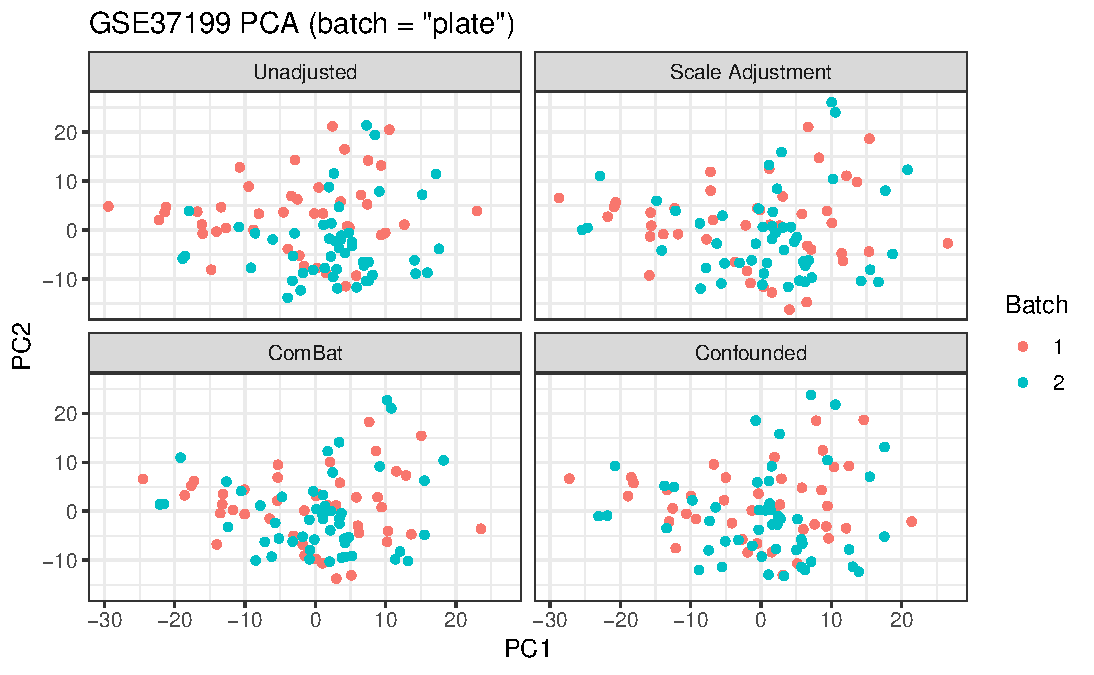
\includegraphics[width=\columnwidth]{figures/final/pca.pdf}
	\caption{\textbf{Principal components analysis} (PCA) of the GSE37199 dataset before and after batch adjustment with various adjusters.
	None of the datasets appear to be linearly separable.
	Confounded appears to maintain the same distribution of data overall as the unadjusted data while perhaps aligning the batches' distributions.}
	\label{fig:pca}
\end{figure}
\begin{figure}
	\centering
	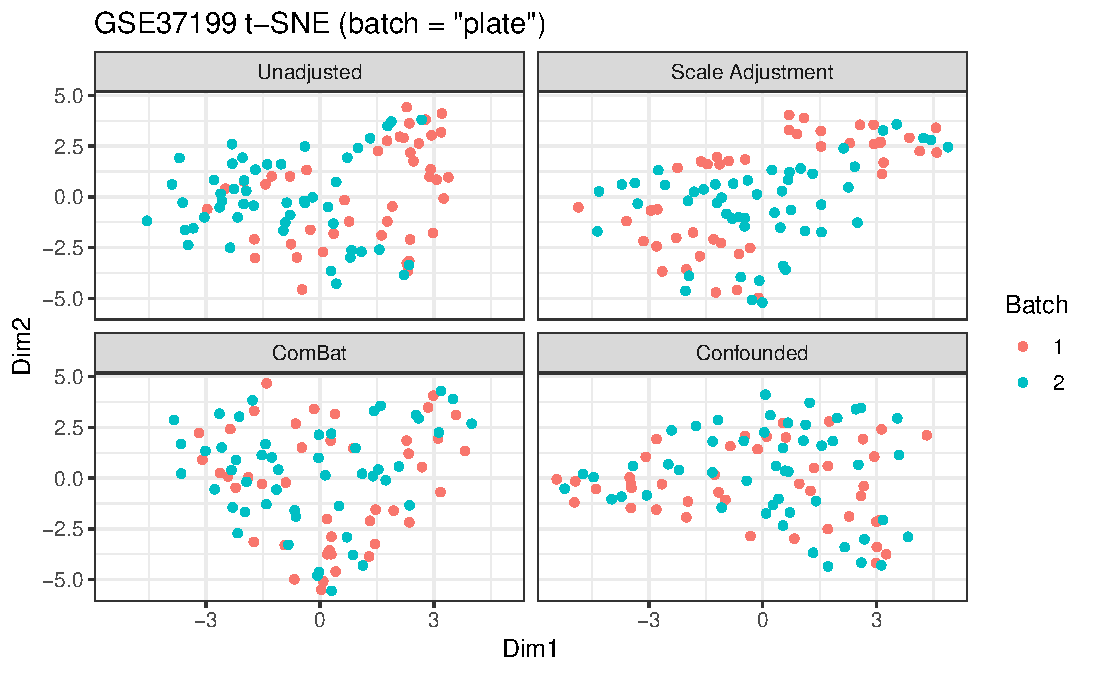
\includegraphics[width=\columnwidth]{figures/final/tsne.pdf}
	\caption{\textbf{T-distributed Stochastic Neighbor Embedding} (t-SNE) plot for the GSE37199 dataset before and after adjustment with several algorithms.
	The data seem to cluster less by batch for both Confounded and ComBat, indicating that both adjusters may be removing nonlinear effects in this dataset.}
	\label{fig:tsne}
\end{figure}

Confounded shows mixed success with the MSE and MMD metrics.
With MSE, Confounded outperformed the scale adjuster in 3 of the 4 datasets by a factor of $\frac{1}{2}$ to $\frac{1}{6}$ but scored drastically higher on the fourth dataset.
With MMD, Confounded outperformed the scale adjuster again in 3 of the 4 datasets, this time by a factor of $\frac{1}{2}$ to $\frac{1}{10}$ and tied the scale adjuster on the fourth dataset.
With both metrics, Confounded consistently performed somewhat more poorly than ComBat.
(See Figures \ref{fig:mse} and \ref{fig:mmd}.)

\begin{figure}
	\centering
	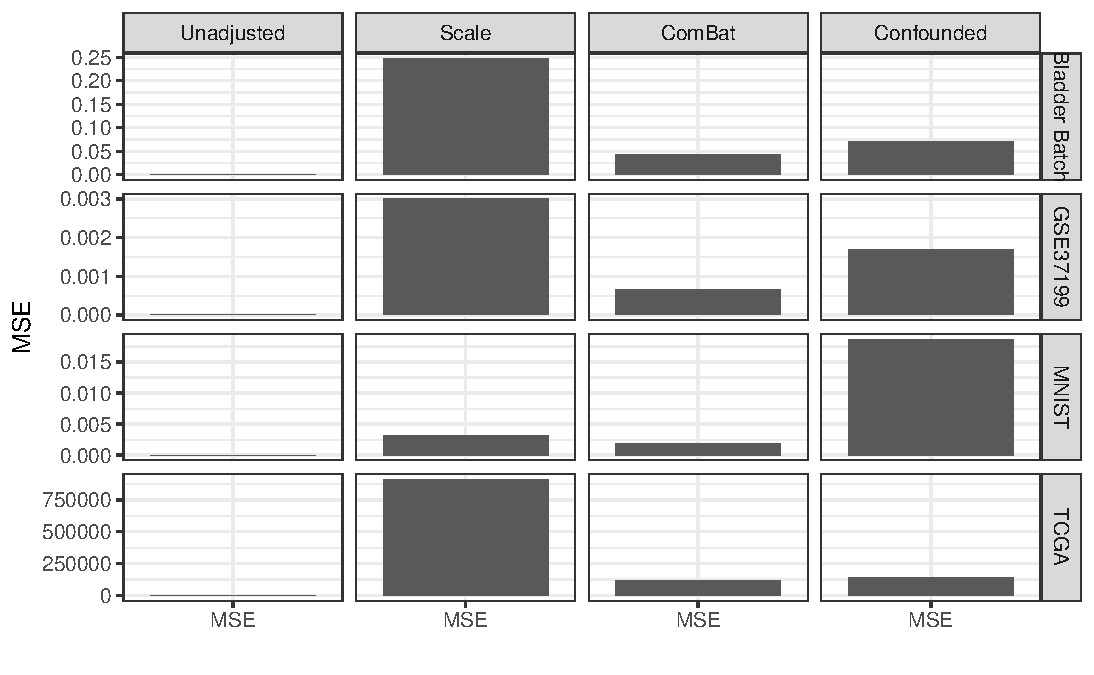
\includegraphics[width=\columnwidth]{figures/final/mse.pdf}
	\caption{\textbf{Mean squared error} (MSE) between the data prior to and after adjustment with various algorithms.
	Lower MSE represents that the adjuster has more faithfully reproduced the input data.
	MSE for unadjusted data will always be 0 because the input data is identical to the output data.
	Confounded usually performs better than the scale adjuster and somewhat worse than ComBat when measuring MSE.}
	\label{fig:mse}
\end{figure}
\begin{figure}
	\centering
	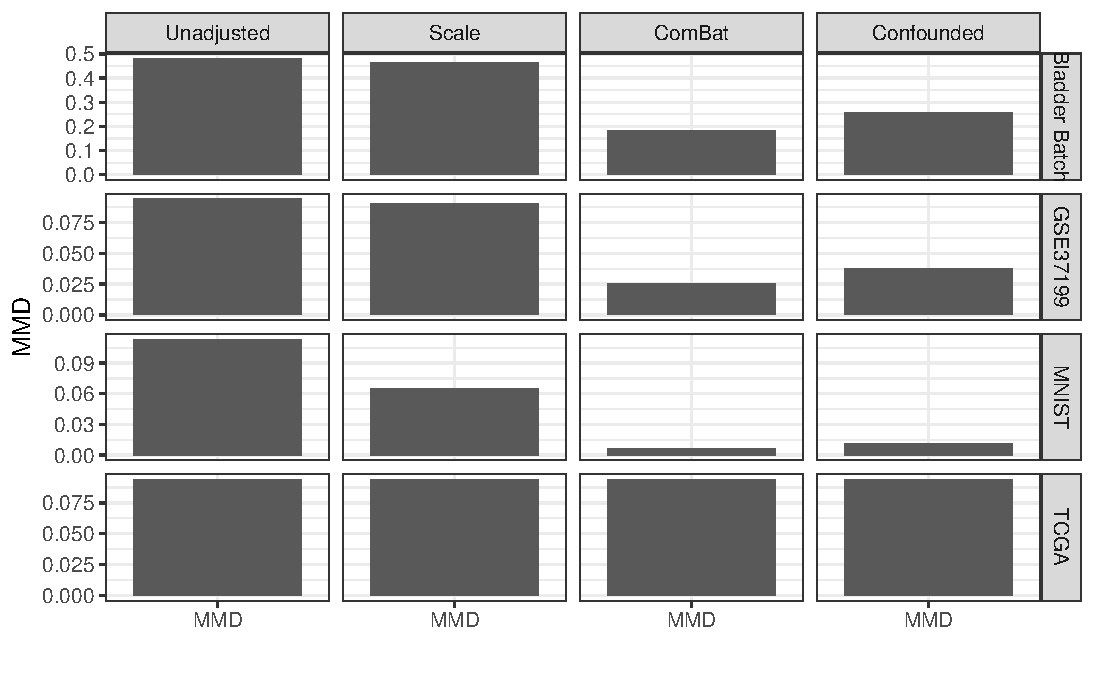
\includegraphics[width=\columnwidth]{figures/final/mmd.pdf}
	\caption{\textbf{Maximum mean discrepancy} (MMD) between different batches. Lower MMD indicates that the distributions of the different batches are more similar.
	In cases with more than two batches, MMD is computed pairwise between each batch and averaged.
	In each case, Confounded usually performs better than the scale adjuster and somewhat worse than ComBat when measuring MSE.}
	\label{fig:mmd}
\end{figure}

We would expect that after batch adjustment by an ideal adjuster, batch would no longer be detectable by any machine learning classifier.
Using the batch classification accuracy metric, Confounded seems to outperform other adjusters on larger datasets, whereas ComBat and Confounded seem to perform about the same on smaller datasets (see Figure \ref{fig:batch}).
With both the bladderbatch and GSE37199 datasets, batch classification accuracy decreases well below baseline after batch adjustment with ComBat for all classifiers we tested (see Table \ref{tab:batch}).
Interestingly, batch accuracy also decreases drastically for the MNIST and TCGA datasets, but only for the Naive Bayes classifier.
This may be due to two factors: both ComBat and Naive Bayes use Bayesian methods, so ComBat may specifically remove the effects that Naive Bayes identifies; and Naive Bayes does not find patterns based on interactions between variables.
Although Naive Bayes is no longer able to identify batch effects in the data after ComBat-adjustment, Random Forests (which does use interactions between variables) still has a very high accuracy for MNIST and an increased accuracy for TCGA.
In contrast, after adjustment by Confounded, the Random Forests algorithm's accuracy decreases more than with any other adjuster for both the MNIST and TCGA datasets.
This indicates that while ComBat's performance may work at least as well as Confounded for smaller expression datasets, Confounded may work better with larger datasets.

\begin{figure}
	\centering
	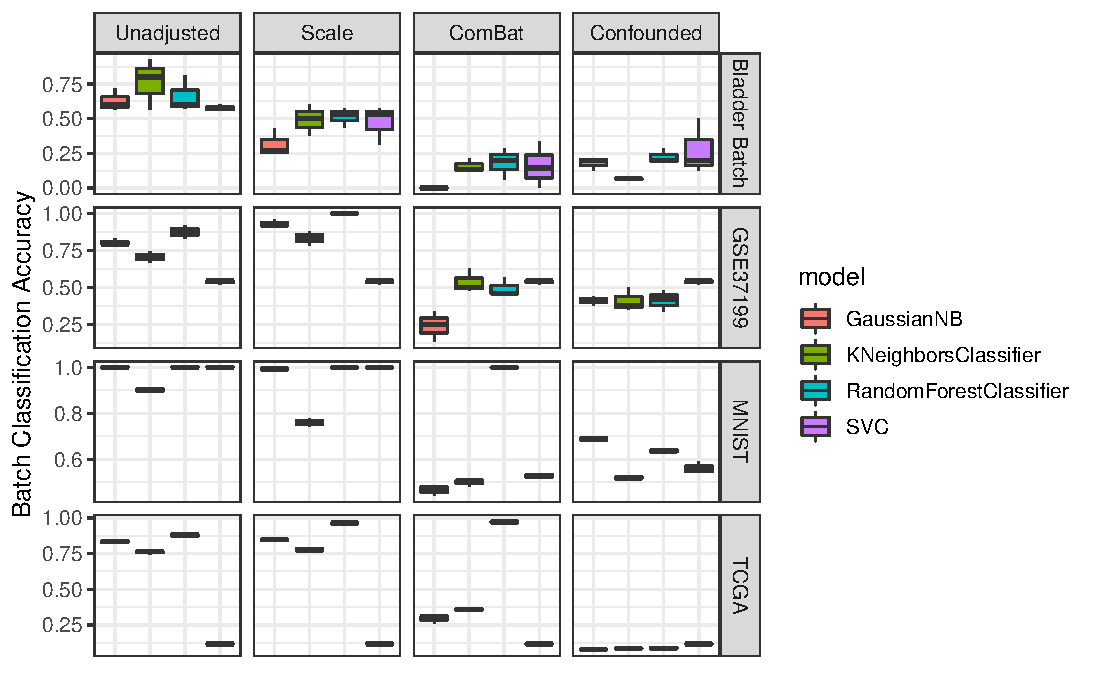
\includegraphics[width=\columnwidth]{figures/final/batch_accuracy.pdf}
	\caption{\textbf{Batch classification accuracy} from 4-fold cross-validation repeated 3 times for several classifiers.
	Lower batch accuracy indicates that more batch-related signal has been removed and therefore indicates better performance.
	Confounded's performance is similar to ComBat's for the smaller datasets and is improved for the larger datasets.
	See also Table \ref{tab:batch}.}
	\label{fig:batch}
\end{figure}
\begin{table}
	\centering
	\centering
\begin{tabular}{l|l|r|r|r}
\hline
Dataset & Adjustment & Baseline & GaussianNB & RandomForest\\
\hline
\rowcolor{gray!6}   & unadjusted &  & 0.626 & 0.688\\
\cline{2-2}
\cline{4-5}
 & scale &  & 0.315 & 0.450\\
\cline{2-2}
\cline{4-5}
\rowcolor{gray!6}   & combat &  & 0.000 & 0.114\\
\cline{2-2}
\cline{4-5}
\multirow[t]{-4}{*}{\raggedright\arraybackslash bladderbatch} & confounded & \multirow[t]{-4}{*}{\raggedleft\arraybackslash 0.333} & 0.386 & 0.315\\
\cline{1-5}
\rowcolor{gray!6}   & unadjusted &  & 0.803 & 0.832\\
\cline{2-2}
\cline{4-5}
 & scale &  & 0.930 & 0.928\\
\cline{2-2}
\cline{4-5}
\rowcolor{gray!6}   & combat &  & 0.238 & 0.423\\
\cline{2-2}
\cline{4-5}
 & confounded &  & 0.338 & 0.353\\
\cline{2-2}
\cline{4-5}
\rowcolor{gray!6}  \multirow[t]{-5}{*}{\raggedright\arraybackslash gse37199} & NA & \multirow[t]{-5}{*}{\raggedleft\arraybackslash 0.538} & 0.662 & 0.670\\
\cline{1-5}
 & unadjusted &  & 0.996 & 1.000\\
\cline{2-2}
\cline{4-5}
\rowcolor{gray!6}   & scale &  & 0.998 & 1.000\\
\cline{2-2}
\cline{4-5}
\multirow[t]{-3}{*}{\raggedright\arraybackslash noisy} & combat & \multirow[t]{-3}{*}{\raggedleft\arraybackslash 0.500} & 0.698 & 1.000\\
\cline{1-5}
\rowcolor{gray!6}   & unadjusted &  & 0.832 & 0.879\\
\cline{2-2}
\cline{4-5}
 & scale &  & 0.846 & 0.965\\
\cline{2-2}
\cline{4-5}
\rowcolor{gray!6}  \multirow[t]{-3}{*}{\raggedright\arraybackslash tcga} & combat & \multirow[t]{-3}{*}{\raggedleft\arraybackslash 0.117} & 0.293 & 0.960\\
\hline
\end{tabular}
	\caption{\textbf{Batch classification accuracy} for several datasets and adjusters.
	The ideal batch adjuster would completely remove all signal due to batch and would therefore \textit{decrease} batch classification accuracy to around the baseline for all classifiers.
	See also Figure \ref{fig:batch}.}
	\label{tab:batch}
\end{table}

With the larger datasets in particular, Confounded outperforms the other adjusters.
On the MNIST dataset, Random Forests is able to detect batch with perfect or near-perfect accuracy after adjustment with the scale adjuster and ComBat, but the highest batch classification accuracy after adjustment by Confounded is Naive Bayes, with an accuracy of 68.8\%.
With TCGA, both the scale adjuster and ComBat drastically increase Random Forests' batch classification accuracy from 87.6\% to 96.3\% and 97.1\% respectively, whereas Confounded decreases the accuracy to 8.8\%.

\subsection{Important signal is still detectable after adjustment by Confounded}

With the smaller datasets, Confounded seems to keep true class information roughly as well as ComBat, (with Random Forests, Bladderbatch: 74.3 for ComBat\% and 72.1\% for Confounded, GSE37199: 60.4\% for ComBat and 69.0\% for Confounded; see Figure \ref{fig:true_class} and Table \ref{tab:true_class}).
For the Bladderbatch dataset, true class accuracy is much lower after adjusting with any algorithm, indicating that cancer status and batch may not be independent.

With the larger datasets, Confounded's true class accuracy consistently decreases below the accuracy of other adjusters.
A look at the MNIST digits before and after adjustment (see Figure \ref{fig:mnist}) shows that Confounded's output is often blurry, as is common with the output of variational autoencoders \cite{hou_deep_2016}.
With MNIST, Confounded's accuracy with Random Forests is still much higher than baseline (84.8\% vs. 11.4\%), but with TCGA, the accuracy decreases below baseline (66.5\% vs. 69.8\%) while the other adjusters' accuracies remain above baseline.
However, preliminary testing indicates that fine-tuning Confounded's parameters to run on these datasets rather than using the default settings may greatly improve Confounded's post-adjustment true class accuracy.
% TODO: include this^

\begin{figure}
	\centering
	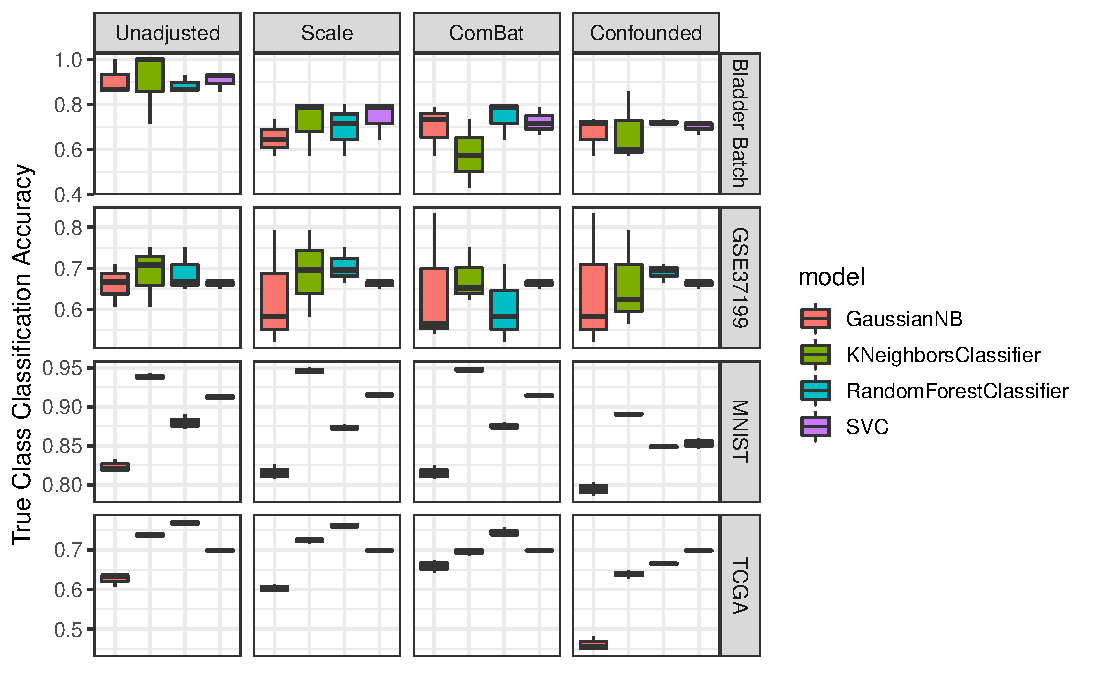
\includegraphics[width=\columnwidth]{figures/final/true_class_accuracy.pdf}
	\caption{\textbf{True class classification accuracy} for several datasets and adjusters with 4-fold cross-validation repeated 3 times.
	See also Table \ref{tab:true_class}.}
	\label{fig:true_class}
\end{figure}
\begin{table}
	\centering
	\centering\rowcolors{2}{gray!6}{white}

\begin{tabular}{l|l|r|r|r|r|r}
\hiderowcolors
\hline
Dataset & Adjustment & Baseline & GaussianNB & KNeighbors & RandomForest & SVC\\
\hline
\showrowcolors
 & Unadjusted &  & 0.9079365 & 0.9047619 & 0.8841270 & 0.9063492\\
\cline{2-2}
\cline{4-7}
 & Scale &  & 0.6492063 & 0.7190476 & 0.6952381 & 0.7428571\\
\cline{2-2}
\cline{4-7}
 & ComBat &  & 0.6968254 & 0.5777778 & 0.7428571 & 0.7222222\\
\cline{2-2}
\cline{4-7}
\multirow[t]{-4}{*}{\raggedright\arraybackslash Bladder Batch} & Confounded & \multirow[t]{-4}{*}{\raggedleft\arraybackslash 0.7017544} & 0.6730159 & 0.6761905 & 0.7206349 & 0.6984127\\
\cline{1-7}
 & Unadjusted &  & 0.6612319 & 0.6890097 & 0.6896135 & 0.6618357\\
\cline{2-2}
\cline{4-7}
 & Scale &  & 0.6322464 & 0.6902174 & 0.7041063 & 0.6618357\\
\cline{2-2}
\cline{4-7}
 & ComBat &  & 0.6467391 & 0.6757246 & 0.6044686 & 0.6618357\\
\cline{2-2}
\cline{4-7}
\multirow[t]{-4}{*}{\raggedright\arraybackslash GSE37199} & Confounded & \multirow[t]{-4}{*}{\raggedleft\arraybackslash 0.6666667} & 0.6461353 & 0.6606280 & 0.6902174 & 0.6618357\\
\cline{1-7}
 & Unadjusted &  & 0.8236658 & 0.9388265 & 0.8801867 & 0.9128345\\
\cline{2-2}
\cline{4-7}
 & Scale &  & 0.8160683 & 0.9462902 & 0.8743188 & 0.9153669\\
\cline{2-2}
\cline{4-7}
 & ComBat &  & 0.8152686 & 0.9478891 & 0.8755154 & 0.9140346\\
\cline{2-2}
\cline{4-7}
\multirow[t]{-4}{*}{\raggedright\arraybackslash MNIST} & Confounded & \multirow[t]{-4}{*}{\raggedleft\arraybackslash 0.1135000} & 0.7944837 & 0.8907100 & 0.8484595 & 0.8528601\\
\cline{1-7}
 & Unadjusted &  & 0.6251933 & 0.7380770 & 0.7675432 & 0.6979360\\
\cline{2-2}
\cline{4-7}
 & Scale &  & 0.6028491 & 0.7232736 & 0.7602833 & 0.6979360\\
\cline{2-2}
\cline{4-7}
 & ComBat &  & 0.6590746 & 0.6953731 & 0.7444855 & 0.6979360\\
\cline{2-2}
\cline{4-7}
\multirow[t]{-4}{*}{\raggedright\arraybackslash TCGA} & Confounded & \multirow[t]{-4}{*}{\raggedleft\arraybackslash 0.6979500} & 0.4612043 & 0.6387186 & 0.6651957 & 0.6979360\\
\hline
\end{tabular}
\rowcolors{2}{white}{white}
	\caption{\textbf{True class classification accuracy} for several datasets and adjusters.
	After adjustment by the ideal batch adjuster, all true class signal should be preserved, and all classifiers should therefore have the same accuracy in predicting true class before and after adjustment.
	See also Figure \ref{fig:true_class}.}
	\label{tab:true_class}
\end{table}

\begin{figure}
	\centering
	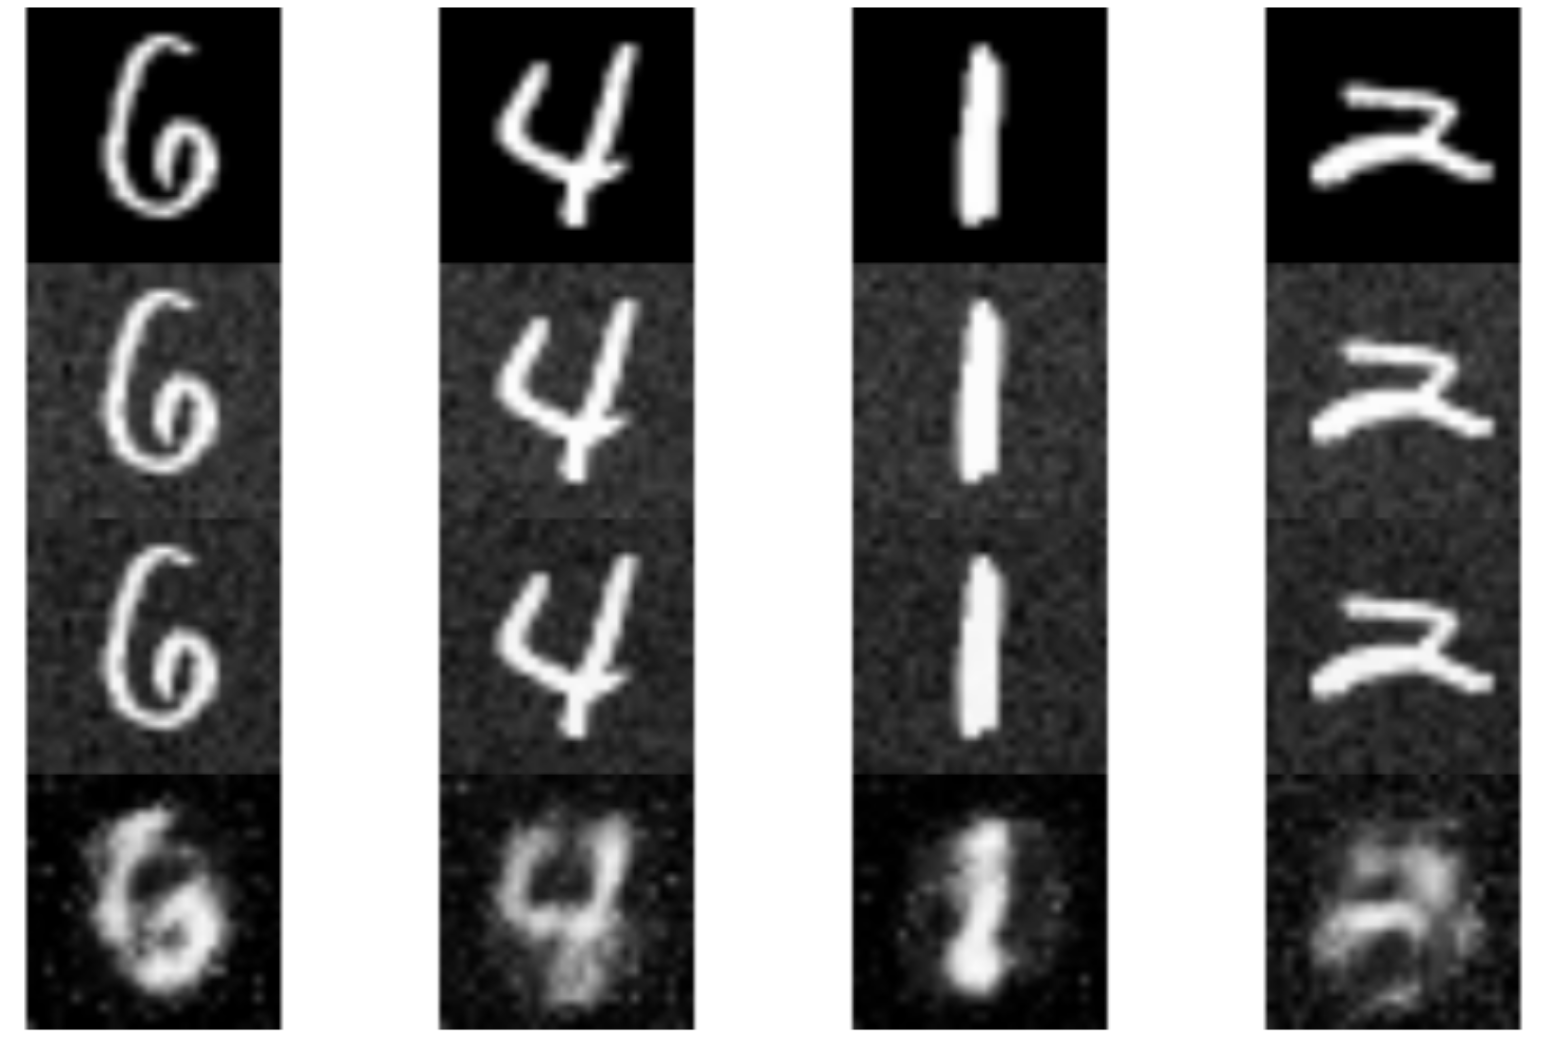
\includegraphics[width=\columnwidth]{figures/rough/mnist.png}
	\caption[]{\textit{TODO: this is old output data and needs to be updated.} \textbf{MNIST handwritten digits}
	\begin{enumerate*}[(a)]
		\item before any adjustment,
		\item with artificial noise added,
		\item adjusted for noise by ComBat, and
		\item adjusted for noise by Confounded.
	\end{enumerate*}
	Although Confounded seems to remove more noise from the background and make it look more like the original background, it struggles in some cases to accurately replicate the input data.}
	\label{fig:mnist}
\end{figure}

\section{Discussion} \label{sec:discussion}

\subsection{Classification accuracy quantifies batch removal more accurately than MSE and MMD}

Our MSE \ref{fig:mse} and MMD \ref{fig:mmd} metrics both show that ComBat performed better than Confounded for the MNIST dataset, but the effects left after ComBat finished are still identifiable by Random Forests with 99.9\% accuracy (Table \ref{tab:batch}).
Additionally, previous work \cite{dayton_classifying_2017-1} has shown that PCA can be misleading when determining whether batch effects have been sufficiently removed from a dataset.
Each of these methods seems to focus on linear separability.

Many machine learning classification algorithms are able to identify both linear and nonlinear interactions between variables.
A decrease in classifier accuracy represents that nonlinear batch effects have been decreased.
Random Forests often has high batch classification accuracy after ComBat-adjustment even when other classifiers are unable to identify differences between batches, whereas SVC often performs no better than baseline (see Figure \ref{fig:batch} and Table \ref{tab:batch}).
In addition, ComBat often excels at hiding batch effects from Naive Bayes.
We suggest that it may be important to use several classifiers to identify whether batch effects remain after correction.

We encourage future researchers who study batch correction or who use it in their pipelines to use classifier accuracy to determine the degree to which batch effects still remain in their data.
This is especially important to take into account when analyses will include some type of machine learning that can detect nonlinear effects.

\subsection{Dataset should be considered when applying batch adjustment}

Nonlinear batch effects often remain after traditional batch adjustment for larger datasets.
For the larger datasets in our study, Confounded outperformed the other batch adjustment algorithms according to the batch classification metrics.
However, Confounded also reduced the amount of true signal in those same datasets more than other algorithms.
This may be able to be ameliorated by hyperparameter optimization,
but in cases where batch effects and true signal are not independent, researchers may need to decide the tradeoff between how much true signal loss and remaining batch effects are acceptable.

\subsection{Confounded may have other uses}

At its root, batch correction is a data integration problem;
data from multiple batches must have batch-specific confounding effects removed in order to be treated as one dataset.
Confounded shows promise in removing traditional batch effects from microarray expression data in the Bladderbatch and GSE37199 datasets.
It also effectively decreased artificial batch effects in image data and tissue-specific effects in RNA-Seq data.
Confounded may be effective in other data integration problems, such as combining microarray with RNA-Seq datasets, or merging several large datasets measured under different conditions.
We invite future researchers to utilize Confounded in any pipelines where data must be integrated from different sources, and to assess the effectiveness of doing so by measuring batch classifier accuracy.

\bibliography{references}

\end{document}
